
%(BEGIN_QUESTION)
% Copyright 2007, Tony R. Kuphaldt, released under the Creative Commons Attribution License (v 1.0)
% This means you may do almost anything with this work of mine, so long as you give me proper credit

Determine how to adjust this bourdon-tube pressure gauge mechanism to correct for the calibration error exhibited in the ``As-Found'' calibration table.  

\vskip 10pt

\hbox{ % Encloses both image and table into a horizontal group

\includegraphics[width=15.5cm]{i02943x01.eps} \hskip 30pt

% No blank lines allowed between lines of an \halign structure!
% I use comments (%) instead, so that TeX doesn't choke.

%$$\vbox{\offinterlineskip
\vbox{\offinterlineskip
\halign{\strut
\vrule \quad\hfil # \ \hfil & 
\vrule \quad\hfil # \ \hfil \vrule \cr
\noalign{\hrule}
%
% First row
Applied pressure & Gauge indication \cr
%
(PSI) & (PSI) \cr
%
\noalign{\hrule}
%
% Another row
0 & 0 \cr
%
\noalign{\hrule}
%
% Another row
25 & 22 \cr
%
\noalign{\hrule}
%
% Another row
50 & 44 \cr
%
\noalign{\hrule}
%
% Another row
75 & 66 \cr
%
\noalign{\hrule}
%
% Another row
100 & 88 \cr
%
\noalign{\hrule}
} % End of \halign 
} % End of \vbox
%}$$ % End of \vbox

} % End of \hbox enclosing both image and table

\vskip 10pt

After inspecting the gauge, you see that you are able to adjust the following things:

\begin{itemize}
\item{} Lenghthen the ``link''
\item{} Shorten the ``link''
\item{} Move the pivot point between the ``link'' and the ``sector'' toward the pinion gear
\item{} Move the pivot point between the ``link'' and the ``sector'' away from the pinion gear
\item{} Shift the pointer clockwise on the ``pinion gear'' shaft
\item{} Shift the pointer counter-clockwise on the ``pinion gear'' shaft
\item{} Bend the bourdon tube upward (straighter)
\item{} Bend the bourdon tube downward (more bent)
\end{itemize}

\vskip 10pt

\noindent
Credit will be given for determining the following:

\begin{itemize}
\item{} Identify which piece of the mechanism to adjust to correct the gauge's calibration, and which way to adjust it (e.g. which direction to adjust the mechanism)
\vskip 5pt
\item{} Explain why this adjustment will work:
\end{itemize}

\underbar{file i02943}
%(END_QUESTION)





%(BEGIN_ANSWER)

\begin{itemize}
\item{} {\bf (5 points)} Identify which piece of the mechanism to adjust -- {\bf Move the pivot point between the ``link'' and the ``sector'' toward the pinion gear}
\vskip 5pt
\item{} {\bf (5 points)} Explain why this adjustment will work: {\bf Right now, the pointer isn't moving far enough for the applied pressure, so we need to increase the amount of displacement multiplication in the mechanism.  By moving the link in (toward the sector gear pivot), it will require less motion of the bourdon tube to produce the same pointer rotation.  Stated another way, the same bourdon tube motion will result in more pointer rotation, which is what we want.}
\end{itemize}

%(END_ANSWER)





%(BEGIN_NOTES)

{\bf This question is intended for exams only and not worksheets!}.

%(END_NOTES)


